% \documentclass{article}
% \usepackage{beamerarticle}
\documentclass{beamer}
% Beamer theme settings
\usetheme{Madrid}
\usecolortheme{default}
\usepackage{amsmath}
\usepackage{tikz}
\usepackage{mathtools}
\usepackage{hyperref}
\usetikzlibrary{intersections}
\usepackage{graphicx}
\usepackage{svg}
% Define commands for vectors
\newcommand{\va}{\mathbf{a}}
\newcommand{\vb}{\mathbf{b}}
\newcommand{\vc}{\mathbf{c}}
\newcommand{\vd}{\mathbf{d}}
\newcommand{\ve}{\mathbf{e}}
\newcommand{\vv}{\mathbf{v}}
\newcommand{\vu}{\mathbf{u}}
\newcommand{\vw}{\mathbf{w}}
\newcommand{\vx}{\mathbf{x}}
\newcommand{\vy}{\mathbf{y}}
\newcommand{\vz}{\mathbf{z}}
\newcommand{\N}{\mathbb{N}}
\newcommand{\Z}{\mathbb{Z}}
\newcommand{\R}{\mathbb{R}}
\newcommand{\Q}{\mathbb{Q}}
\newcommand{\rank}{\text{rank}}







% Title page

\title[Lecture 5]{Limit, Derivative, Extrema of a Function}
\author[Aprikyan, Tarkhanyan]{Hayk Aprikyan, Hayk Tarkhanyan}
\institute[ACA]{Armenian Code Academy}
\date{November 11, 2024}

\begin{document}

\begin{frame}
  \titlepage
\end{frame}


% slide 1: bounds
\begin{frame}{Bounds}
Suppose we have some set $A$.
\pause
    \begin{block}{Definition}
    We say that
        \begin{itemize}
            \item $a\in\R$ is a lower bound for the set $A$ if $a\leq x$ for every $x$ in $A$.
            \item $b\in\R$ is an upper bound for the set $A$ if $x \leq b$ for every $x$ in $A$.
        \end{itemize}
    \end{block}
\pause
    \begin{exampleblock}{Example}
        Consider the set $A = (3, 9.4]=\{x\in \R \:\vert\: 3<x\le 9.4\}$.

        \begin{itemize}
            \item $-1, 2, 3$ are lower bounds for $A$.
            \item $9.4, 10.1, 400$ are upper bounds for $A$.
        \end{itemize}
    \end{exampleblock}
\pause
    \begin{block}{Definition}
        If a set has both upper and lower bounds, it is \textbf{bounded}.
    \end{block}
\end{frame}


% slide 1: bounds
\begin{frame}{Bounds}
    \begin{block}{Definition}
        \begin{itemize}
            \item The largest real number that is a lower bound for $A$ is called the \textbf{infimum} of $A$ and denoted $\inf(A)$.
            
            \item The smallest real number that is an upper bound for $A$ is called the \textbf{supremum} of $A$ and denoted $\sup(A)$.
            
        \end{itemize}
    \end{block}
\pause

    \begin{exampleblock}{Example}
        For the set $A = (3, 9.4]$, $\inf(A)=3, \: \sup(A)=9.4$.
    \end{exampleblock}
\pause

    \begin{block}{Remark}
        The supremum and infimum may or may not belong to the set itself.
    \end{block}
    If the supremum (infimum) belongs to the set, we call it the \textbf{maximum} \textbf{(minimum)}.
\end{frame}


% slide 1: bounds
\begin{frame}{Bounds}
    \begin{block}{Remark}
        A real number $a$ is the infimum of a set $A$ if and only if:
        \begin{enumerate}
            \item $a \le x$ for every $x\in A$,
            \item For every positive number $\varepsilon>0$ there exists an element $x_0\in A$ such that $a+\varepsilon > x_0$.
        \end{enumerate}
    \end{block}
    \pause
    
    \begin{block}{Remark}
        A real number $b$ is the supremum of a set $A$ if and only if:
        \begin{enumerate}
            \item $b \ge x$ for every $x\in A$,
            \item For every positive number $\varepsilon>0$ there exists an element $x_0\in A$ such that $b-\varepsilon < x_0$.
        \end{enumerate}
    \end{block}
    % \pause
    % This means that $\inf(A)$ is the \textit{}
\end{frame}




% slide 2: limits
\begin{frame}{Limit of a Sequence}
 Let $\{a_n\}$ be a sequence of real numbers. \pause
    \begin{block}{Definition}
       We say that the sequence $\{a_n\}$ converges to a limit $L$, denoted as $$\lim\limits_{n \to \infty} a_n = L,$$ if for every positive number $\varepsilon>0$, there exists a positive integer $N$ such that for all $n \geq N$, the terms of the sequence satisfy $$|a_n - L| < \varepsilon.$$
    \end{block}

    In other words, for any positive number, the terms eventually get close to $L$ by less than that number.
    \pause
        \begin{block}{Definition}
       If $\{a_n\}$ has a \textit{finite} limit we say that it is \textbf{convergent}, otherwise it is \textbf{divergent}.
    \end{block}

\end{frame}
 
% slide 2: limits
\begin{frame}{Limit of a Sequence}
    \begin{exampleblock}{Example}
        Consider the sequence $\{ \frac{1}{n} \}$. We claim that $\lim\limits_{n \to \infty} \frac{1}{n} = \pause0$.

        \pause Proof: For any $\varepsilon > 0$, choose $N$ such that $\frac{1}{N} < \varepsilon$. Then, for all $n \geq N$, we have
        \[
        \left| \frac{1}{n} - 0 \right| = \frac{1}{n} < \frac{1}{N} < \varepsilon.
        \]
        Therefore, the sequence converges to $0$, as $n$ approaches infinity.
    \end{exampleblock}
\pause

    \begin{exampleblock}{Example}
        Consider the sequence $\left\{ (\frac{2}{3})^n \right\}$. $\lim\limits_{n \to \infty} (\frac{2}{3})^n  = 0$.

    \end{exampleblock}
    \pause

    \begin{exampleblock}{Example}
        Consider the sequence $\left\{ 0.3n \right\}$. $\lim\limits_{n \to \infty} 0.3n  = \infty$ (it is divergent).

    \end{exampleblock}

\end{frame}


% slide 2: limits
\begin{frame}{Limit of a Sequence}

    \begin{block}{Properties}
\begin{enumerate}[<+->]
    \item        If $\lim\limits_{n \to \infty} a_n = L$ and $\lim\limits_{n \to \infty} b_n = M$, then
        \[
        \lim\limits_{n \to \infty} (a_n + b_n) = L + M
        \]
% \item        If $\lim\limits_{n \to \infty} a_n = L$ and $\lim\limits_{n \to \infty} b_n = M$, then
        \[
        \lim\limits_{n \to \infty} (a_n \cdot b_n) = L \cdot M
        \]
% \item        If $\lim\limits_{n \to \infty} a_n = L$ and $\lim\limits_{n \to \infty} b_n = M$ (where $M \neq 0$), then
        \[
        \lim\limits_{n \to \infty} \frac{a_n}{b_n} = \frac{L}{M}  \text{ (if $M\ne0$)}
        \]
\item        If $\lim\limits_{n \to \infty} a_n = L$, then for any constant $c$, 
        \[
        \lim\limits_{n \to \infty} (c \cdot a_n) = c \cdot L.
        \]
\item        If $a_n \leq b_n \leq c_n$ for all $n$ and $\lim\limits_{n \to \infty} a_n = \lim\limits_{n \to \infty} c_n = L$, then $\lim\limits_{n \to \infty} b_n = L$.
\end{enumerate} 
\end{block}
\end{frame}



% slide 2: limits
\begin{frame}{Limit of a Function}

Suppose we have a function $f(x)$ and a sequence $x_n$ such that $\lim\limits_{n\to\infty} x_n = a$. Let's plug in the values $x_n$ into $f(x)$: $y_n = f(x_n)$.
% \bigskip \newline
\pause  Now let's take another sequence $\tilde{x}_n$ that tends to $a$ and set $\tilde{y}_n=f(\tilde{x}_n)$. \pause Then another, then another... \pause If \textbf{for all sequences} $x_n\to a$, the sequence $y_n$ converges to a certain limit: $\lim\limits_{n\to\infty} y_n =A$, we say that $\lim\limits_{x\to a} f(x) = A$.
% \bigskip
\pause \newline In other words, if the value of $f(x)$ always approaches $A$, as its input approaches to $a$, we say that $\lim\limits_{x\to a} f(x) = A$.

\pause

\begin{example}
Let $f(x) = \frac{1}{x}$. For every $x_n \to 3$, the limit of $f(x_n)$ is $\frac{1}{3}$, therefore $\lim\limits_{x\to 3} f(x)=\frac{1}{3}$. Meanwhile, it has no limit when $x\to 0$.
\end{example} \pause
% An equivalent definition would be: We say that $\lim\limits_{x\to a}f(x)=A$ if for every positive number $\varepsilon>0$, there exists a positive number $\delta>0$, such that for all $x$, if $0<|x-a|<\delta$ then $|f(x)-A| < \varepsilon.$
\begin{definition}
    We say that $\lim\limits_{x\to a}f(x)=A$ if for every $\varepsilon>0$, there exists a positive number $\delta>0$, such that for all $x$, if $0<|x-a|<\delta$ then $|f(x)-A| < \varepsilon.$
\end{definition}

\end{frame}



% slide 2: limits
\begin{frame}{Limit of a Function}

      \begin{center}

    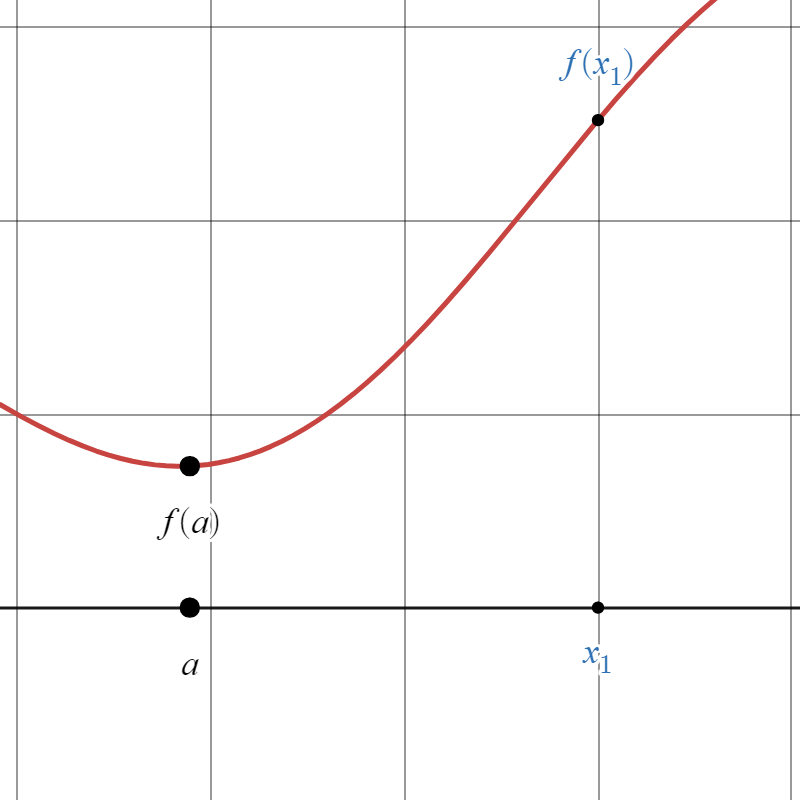
\includegraphics[height=0.75\textheight, keepaspectratio]{cont1.png}
  \end{center}

{\color{white} As we see, $\lim\limits_{x\to a} f(x) = f(a)$.}

\end{frame}


% slide 2: limits
\begin{frame}{Limit of a Function}

      \begin{center}

    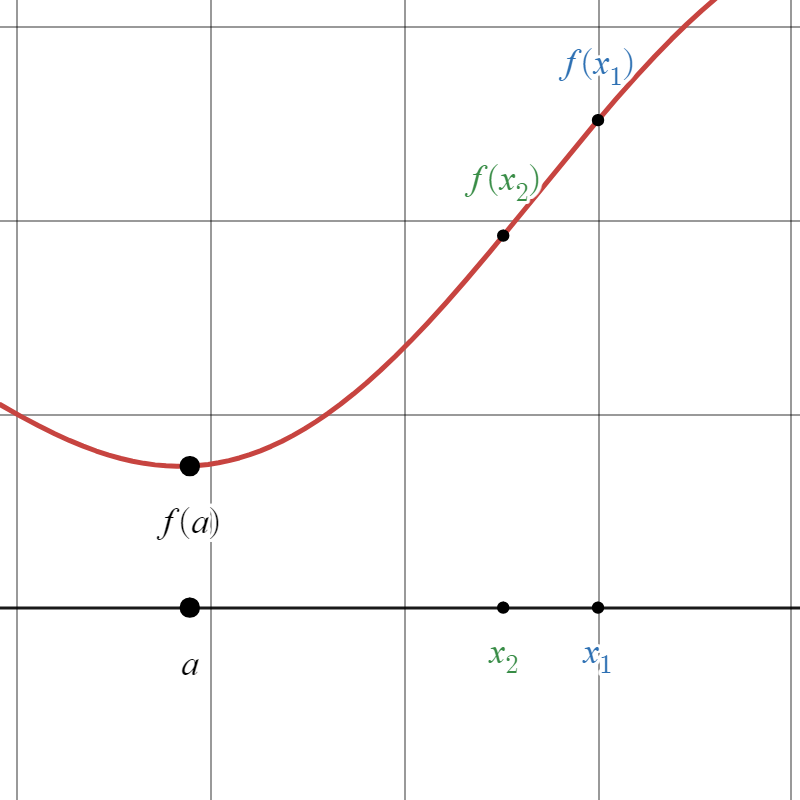
\includegraphics[height=0.75\textheight, keepaspectratio]{cont2.png}
  \end{center}

{\color{white} As we see, $\lim\limits_{x\to a} f(x) = f(a)$.}

\end{frame}


% slide 2: limits
\begin{frame}{Limit of a Function}

      \begin{center}

    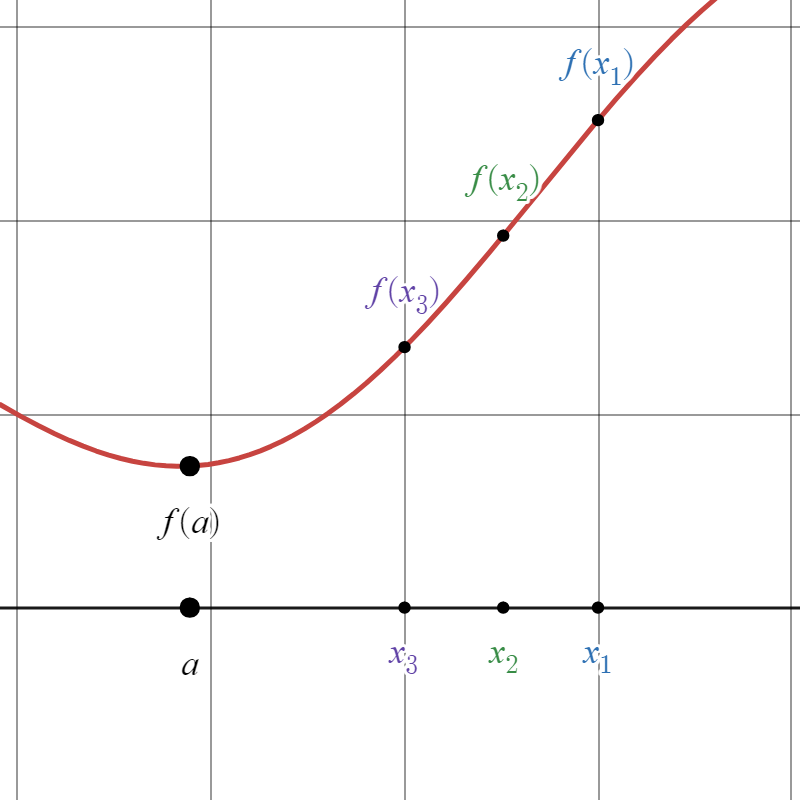
\includegraphics[height=0.75\textheight, keepaspectratio]{cont3.png}
  \end{center}

{\color{white} As we see, $\lim\limits_{x\to a} f(x) = f(a)$.}

\end{frame}


% slide 2: limits
\begin{frame}{Limit of a Function}

      \begin{center}

    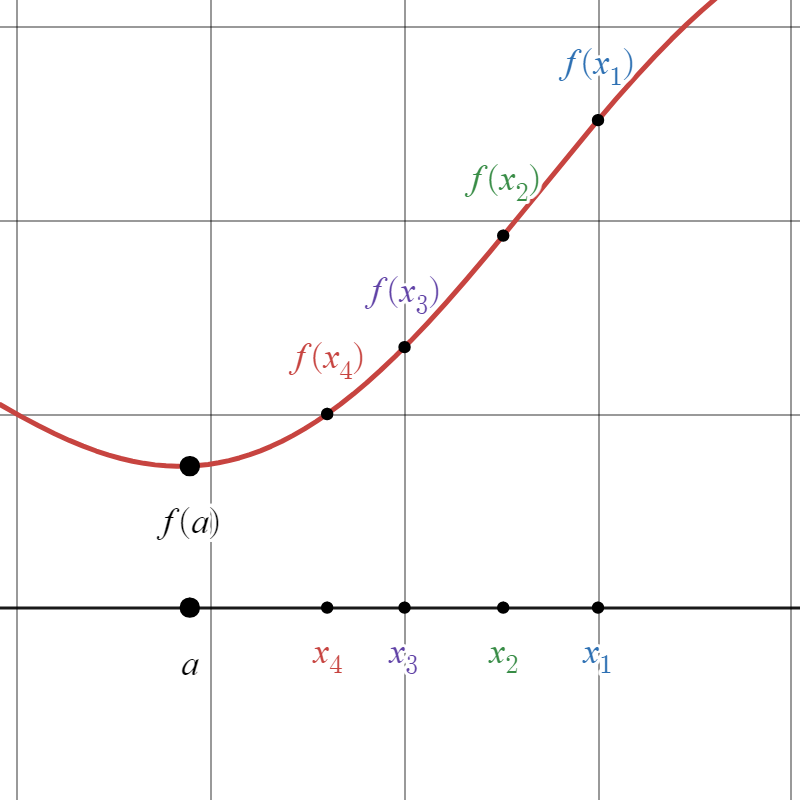
\includegraphics[height=0.75\textheight, keepaspectratio]{cont4.png}
  \end{center}

{\color{white} As we see, $\lim\limits_{x\to a} f(x) = f(a)$.}

\end{frame}


% slide 2: limits
\begin{frame}{Limit of a Function}

      \begin{center}

    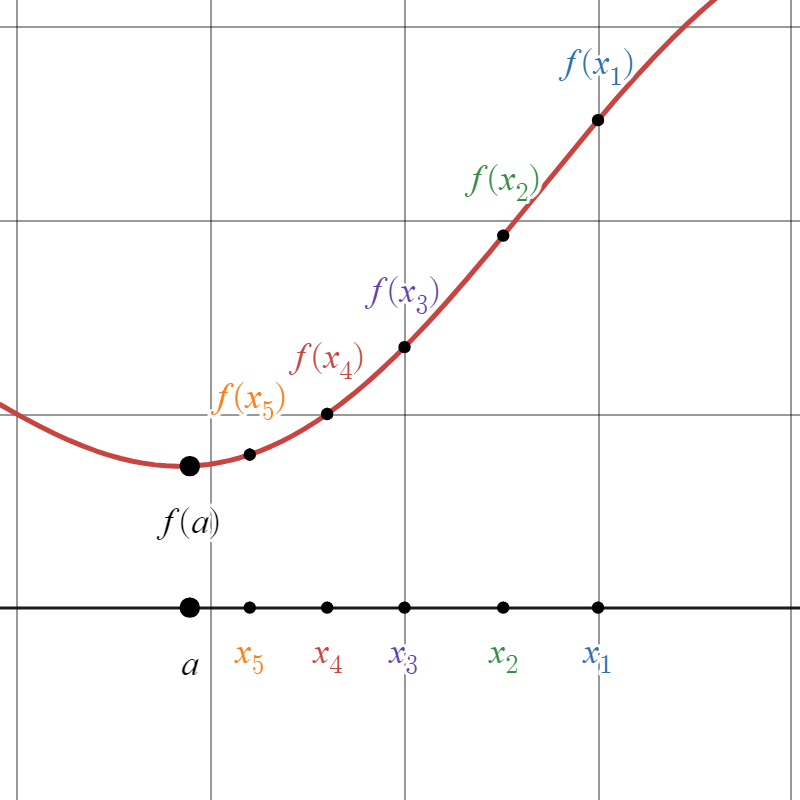
\includegraphics[height=0.75\textheight, keepaspectratio]{cont5.png}
  \end{center}\pause

  As we see, $\lim\limits_{x\to a} f(x) = f(a)$.


\end{frame}




% slide 3: cont
\begin{frame}{Continuity}
    \begin{block}{Definition}
        A function $f(x)$ is said to be \textbf{continuous at a point} $c$ if the following three conditions are satisfied:
        \begin{enumerate}
            \item $f(c)$ is defined.
            \item $\lim\limits_{x \to c} f(x)$ exists.
            \item $\lim\limits_{x \to c} f(x) = f(c)$.
        \end{enumerate}
    \end{block}
\pause
    \begin{exampleblock}{Example}
        The function $f(x) = \frac{1}{x}$ is continuous for all $x$ in its domain except at $x = 0$.
    \end{exampleblock}
\pause
    \begin{block}{Definition}
        If a function is continuous at every point in its domain, it is called a \textbf{continuous function}.
    \end{block}
\end{frame}

% slide 3: cont
\begin{frame}{Continuity}
      \begin{center}

    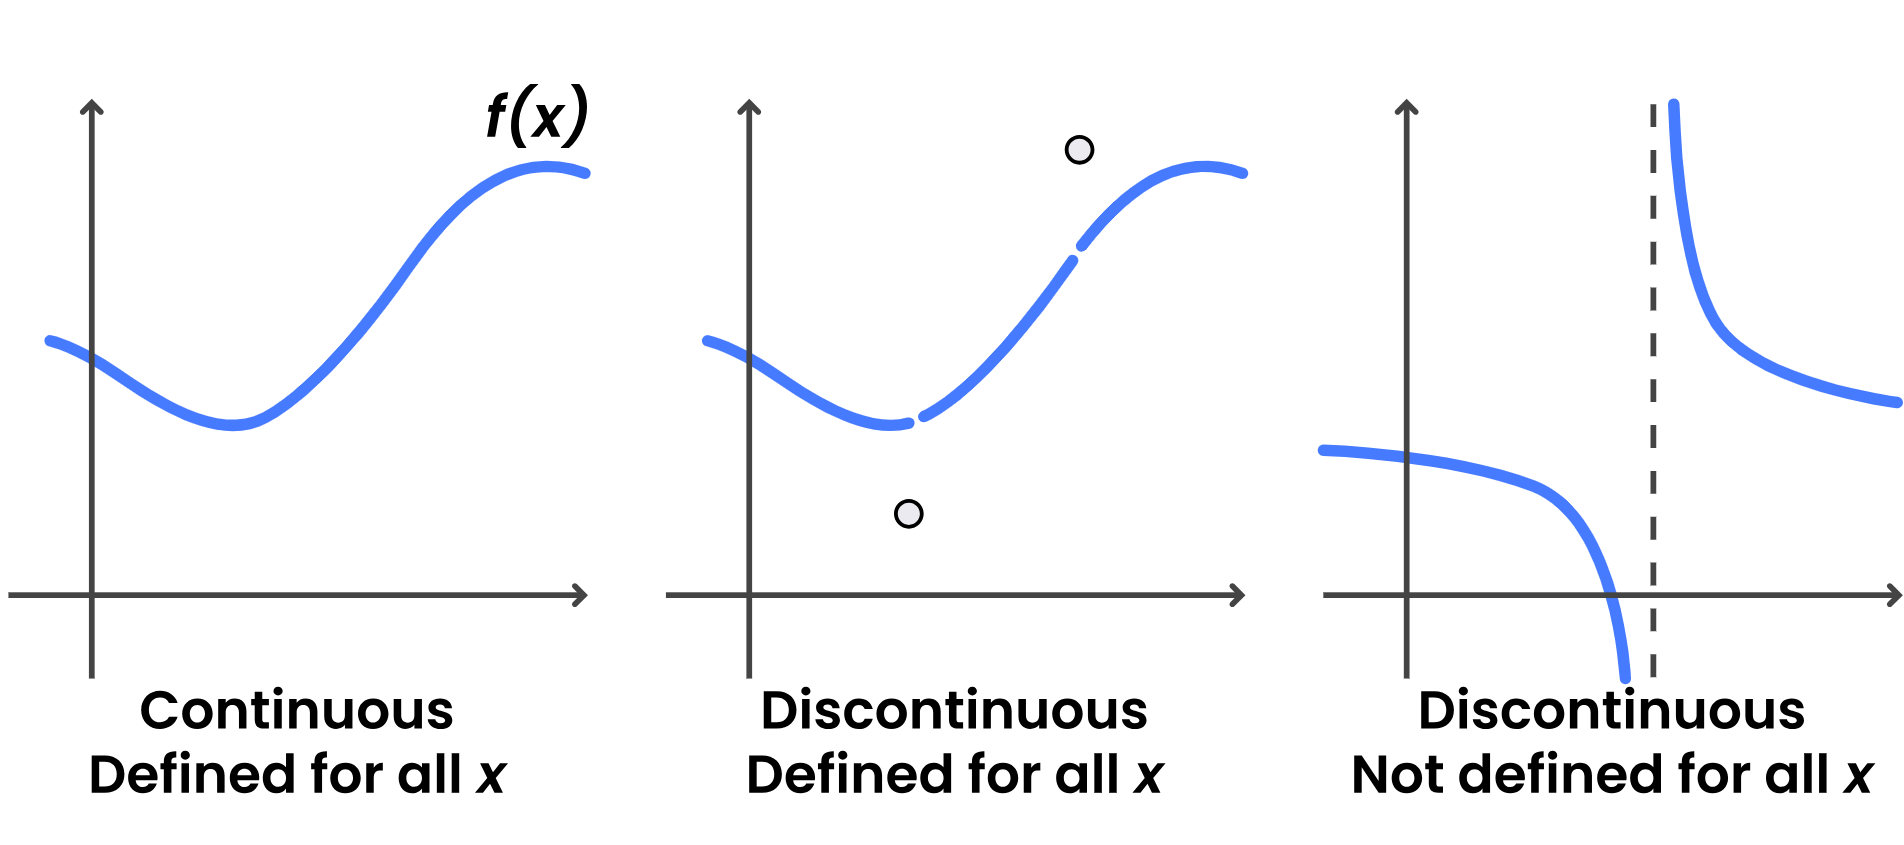
\includegraphics[width=\textwidth, height=\textheight, keepaspectratio]{cont.png}
  \end{center}
\end{frame}


% slide 3: cont
\begin{frame}{Continuity}
   \begin{block}{Properties}
       If \(f\) and \(g\) are continuous at \(a\), and \(c\) is a constant, then the following functions are also continuous at \(a\):

\begin{itemize}
    \item \(f \pm g\)
    \item \(cf\)
    \item \(fg\)
    \item \(\frac{f}{g}\) (if \(g(a) \neq 0\))
\end{itemize}
   \end{block}
   \pause
   \begin{exampleblock}{Example}
   The following functions are continuous \textit{in their domains}: 
     \begin{itemize}
         \item Polynomials (e.g. $x^2+7x-1, \: xy-y^4+z$)
         \item Root functions (e.g. $\sqrt{x}, \sqrt[5]{x}$)
         \item Exponential and logarithmic functions (e.g. $2^x, e^{3x}$, $\ln{x}$)
         \item Trigonometric functions and their inverses (e.g. $\cos(3x), \arcsin{x}$)
     \end{itemize}
   \end{exampleblock}
\end{frame}

% slide 4: derivative
\begin{frame}{Derivative}
Let $X \subset \R$ be a subset of real numbers and $f:X\to\R$ be any function.
    \begin{block}{Definition}
        It is said $f(x)$ is \textbf{differentiable at a point} $a\in X$, if the following limit
        \[
  \lim_{{h \to 0}} \frac{f(a + h) - f(a)}{h}
        \]
        or, equivalently,
        \[
  \lim_{{x\to a}} \frac{f(x) - f(a)}{x-a}
        \]
         exists and is finite. Then it is denoted by $f'(a)$ or $\dfrac{df}{dx}(a)$ and is called the \textbf{derivative} of the function $f(x)$ at the point $a$.
    \end{block}
\pause
    \begin{block}{Definition}
        A function $f(x)$ is said to be \textbf{differentiable on a set} $A$ if it is differentiable at every point of $A$.
    \end{block}
\end{frame}


% slide 4: derivative
\begin{frame}{Derivative}
    \begin{exampleblock}{Example}
        Consider the function $f(x) = x^2$. The derivative of $f(x)$ is:
        \[
        f'(x) = \lim\limits_{{h \to 0}} \frac{(x + h)^2 - x^2}{h} = \lim\limits_{{h \to 0}} \frac{x^2+2xh+h^2 - x^2}{h} = 2x
        \]
        Thus, $f(x)$ is differentiable everywhere, and its derivative is $f'(x) = 2x$.
    \end{exampleblock}
\pause
    \begin{block}{Remark}
        If a function is differentiable on an interval, it is also continuous on that interval, but the reverse is not necessarily true.
    \end{block}
        \begin{exampleblock}{Example}
        The function $f(x)=|x|$ is continuous everywhere but it is not differentiable at point $x=0$.
    \end{exampleblock}
\end{frame}



% slide 4: derivative
\begin{frame}{Derivative}
We denote the derivative of $f'(x)$ by $f''(x)$, that of $f''(x)$ by $f'''(x)$, etc. The derivative taken of $f(x)$ $n$ times is also denoted by $f^{(n)}(x)$.\pause

For any differentiable functions $f, g$ and a real number $c$, the following rules hold:
    \begin{block}{Properties}
\begin{enumerate}[<+->]
    \item    $(cf)'=c\cdot f'$
    \item    $(f \pm g)'=f'\pm g'$
    \item    $(fg)'=f'g+fg'$
    \item    $\left(\dfrac{1}{f}\right)'=-\dfrac{f'}{f^2}$, if $f\ne 0$
    \item    $\left(\dfrac{f}{g}\right)'=\dfrac{f'g-fg'}{g^2}$, if $g\ne 0$
    \item    $(f(g(x)))'=f'(g(x)) \cdot g'(x)$
    % \item    $\left(\dfrac{f}{g}\right)'=\dfrac{f'g-fg'}{g^2}$, if $g\ne 0$
\end{enumerate} 
\end{block}
\end{frame}


% slide 4: derivative
\begin{frame}{Derivative}
     \begin{itemize}[<+->]
         \item The derivative of any constant $f(x)=c$ is:
         \[(c)' = 0\]
         \item The derivative of $f(x)=x$ is:
         \[(x)' = 1\]
         \item The derivative of $f(x)=x^2$ is:
         \[(x^2)' = 2x\]
         \item For any constant $n$, the derivative of $f(x)=x^n$ is:
         \[(x^n)' = nx^{n-1}\]
     \end{itemize}
\end{frame}

% slide 4: derivative
\begin{frame}{Derivative}
     \begin{itemize}[<+->]
         \item The derivative of $f(x)=e^x$ is:
         \[(e^x)' = e^x\]
         \item The derivative of $f(x)=a^x$ is:
         \[(a^x)' = a^x\ln a\]
         \item The derivative of $f(x)=\ln x$ is:
         \[(\ln x)' = \dfrac{1}{x}\]
         \item The derivative of $f(x)=\sin x$ is:
         \[(\sin x)'=\cos x\]
         \item The derivative of $f(x)=\cos x$ is:
         \[(\cos x)'=-\sin x\]
     \end{itemize}
\end{frame}


% % slide 4: derivative
% \begin{frame}{Derivative}
%     Derivatives can be also when calculating a limit of 
% \end{frame}


% slide 4: derivative
\begin{frame}{Derivative}
The derivative of a function at a given point shows the \textbf{"speed" of the function} at that point, the sensitivity of change of its output with respect to its input. \pause In particular,
\begin{block}{Theorem}
    If $f'(a) > 0$ then the function $f$ is increasing at point $a$. That is, there exists a positive number $\delta >0$ such that 
    \begin{center}
        $f(a)>f(x)\quad\text{ for any }x\in(a-\delta,a),$ \\ $f(a)<f(x)\quad\text{ for any }x\in(a,a+\delta). $
    \end{center}
\end{block}\pause
\begin{block}{Theorem}
    If $f'(a) \ge 0$ then the function $f$ is non-decreasing at point $a$. That is, there exists a positive number $\delta >0$ such that  
    \begin{center}
        $f(a) \ge f(x)\quad\text{ for any }x\in(a-\delta,a),$ \\ $f(a)\le f(x)\quad\text{ for any }x\in(a,a+\delta). $
    \end{center}
\end{block}
\end{frame}


% slide 4: derivative
\begin{frame}{Derivative}
\begin{block}{Theorem}
    If $f'(a) < 0$ then the function $f$ is decreasing at point $a$. That is, there exists a positive number $\delta >0$ such that $$ f(a)<f(x)\quad\text{ for any }x\in(a-\delta,a),$$$$f(a)>f(x)\quad\text{ for any }x\in(a,a+\delta). $$
\end{block}
\begin{block}{Theorem}
    If $f'(a) \le 0$ then the function $f$ is non-increasing at point $a$. That is, there exists a positive number $\delta >0$ such that \[ f(a)\le f(x)\quad\text{ for any }x\in(a-\delta,a),\]\[ f(a) \ge f(x)\quad\text{ for any }x\in(a,a+\delta). \]
\end{block}\pause
What if $f'(a)=0$?
\end{frame}


% slide 5: extrema
\begin{frame}{Extrema of a Function}
Let \(f : X \to \mathbb{R}\) be any function.
\begin{block}{Definition}
     \(x_0\in X\) is called a \textbf{local maximum (minimum) point} of \(f\), if there exists \(\delta > 0\) such that for any \(x \in (x_0 - \delta, x_0 + \delta)\cap X\), 
     \[f(x) \leq f(x_0)\]
     \[(f(x) \geq f(x_0))\]
\pause and $f(x_0)$ is called a \textbf{local maximum (minimum)}.
\end{block}

\pause Together, local minimum and maximum points are called local extremum points.
\end{frame}


% slide 5: extrema
\begin{frame}{Extrema of a Function}
     \begin{block}{Definition}
     \(x_0\in X\) is called a \textbf{(global) maximum (minimum) point} of \(f\), if for any \(x \in X\), 
     \[f(x) \leq f(x_0)\]
     \[(f(x) \geq f(x_0))\]
\pause and $f(x_0)$ is called a \textbf{(global) maximum (minimum)}.
\end{block}
\pause Together, global minimum and maximum points are called global extremum points.
\pause Apparently, every global extremum point is also a local extremum point (and the converse is not true).
\end{frame}

% slide 5: extrema
\begin{frame}{Extrema of a Function}

\begin{center}

    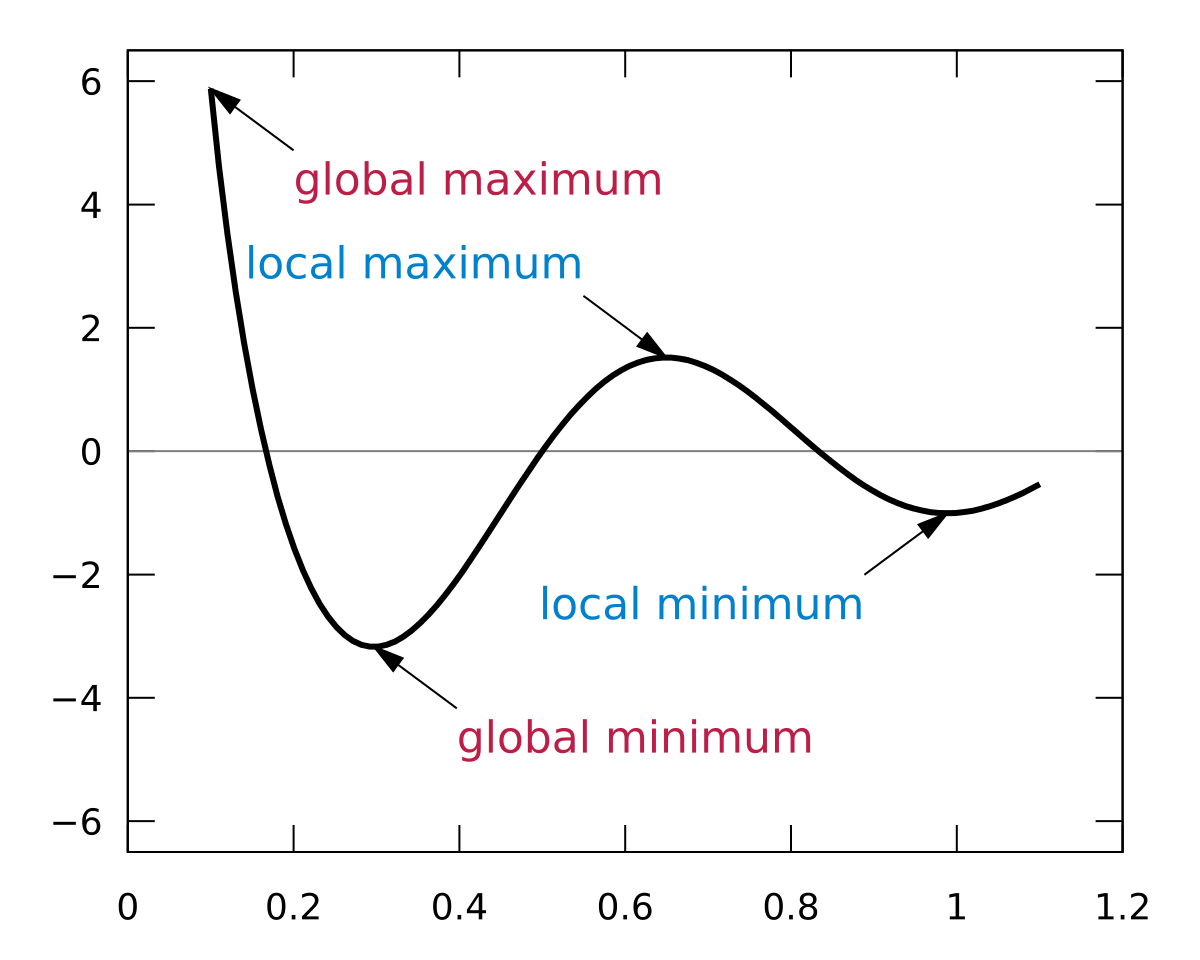
\includegraphics[ height=0.85\textheight, keepaspectratio]{extr2.png}
  \end{center}
\end{frame}

% slide 5: extrema
\begin{frame}{Extrema of a Function}

% \begin{center}
\begin{exampleblock}{Example}
    Which points are the local extremum points of the following functions? \\ \bigskip
% \\\includesvg[ width=0.31\textwidth, keepaspectratio]{image-295}\pause 
 \includesvg[ width=0.31\textwidth, keepaspectratio]{image-296}\pause
 \includesvg[ width=0.31\textwidth, keepaspectratio]{image-297}\pause
 \includesvg[ width=0.31\textwidth, keepaspectratio]{image-290}
\end{exampleblock}
  % \end{center}
\pause
\begin{block}{Theorem}
If a function \(f\) is continuous on a \textit{closed interval} \([a, b]\), then \(f\) has both a global maximum and a global minimum on \([a, b]\).
    
\end{block}

  
\end{frame}

% slide 5: extrema
\begin{frame}{Extrema of a Function}


\begin{block}{Theorem}
If \(x_0\) is an extremum point of \(f\) and there exists \(f'(x_0)\), then \(f'(x_0) = 0\).

\end{block}
\pause

\begin{example}
    Consider the function $f_1(x)=x^2$ which has a minimum at $x=0$.
    \[ f_1'(x)=2x ,\qquad f_1'(0)=0 \]
    \pause Moreover, the function $f_2(x)=-x^2$ has a maximum at $x=0$ and again:
    \[ f_2'(x)=-2x ,\qquad f_2'(0)=0 \]
\pause The function $f_3(x)=x^3$ has no local extremum point, yet    
    \[ f_3'(x)=3x^2 ,\qquad f_2'(0)=0 \]
\end{example}
  \pause Hence, the condition $f'(x)=0$ is necessary but \textit{not sufficient}.
\end{frame}


% slide 5: extrema
\begin{frame}{Extrema of a Function}

Let \(f : X \to \mathbb{R}\) be any function.

\begin{block}{Definition}
$x_0 \in X$ is called a \textbf{critical point} if $f'(x_0)$ doesn't exist or $f'(x_0)=0$.

\end{block}
\pause
How can we tell if a critical point is (or isn't) a local minimum/maximum point?
\end{frame}


% slide 5: extrema
\begin{frame}{Extrema of a Function}
\begin{block}{Theorem 1}
If \(f'(x_0) = 0\) and there exists finite \(f''(x_0)\), then

\begin{enumerate}
    \item If \(f''(x_0) > 0\), then \(x_0\) is a local minimum point,
    \item If \(f''(x_0) < 0\), then \(x_0\) is a local maximum point.
\end{enumerate}


\end{block}
\pause
\begin{block}{Theorem 2}
If for some $\delta >0$, $\(f\) is differentiable in the intervals \((x_0 - \delta, x_0)\) and \((x_0, x_0 + \delta)\) and continuous at \(x_0\), then

\begin{enumerate}
    \item If \(f'(x) > 0\) for \(x \in (x_0 - \delta, x_0)\) and \(f'(x) < 0\) for \(x \in (x_0, x_0 + \delta)\), then \(x_0\) is a local maximum point.
    \item If \(f'(x) < 0\) for \(x \in (x_0 - \delta, x_0)\) and \(f'(x) > 0\) for \(x \in (x_0, x_0 + \delta)\), then \(x_0\) is a local minimum point.
    \item If \(f'(x)\) doesn’t change its sign, then \(x_0\) is not an extremum point.
\end{enumerate}



\end{block}
\end{frame}



% slide 5: extrema
\begin{frame}{Extrema of a Function}
Wrapping up, how can we use our knowledge to find the local extrema of a given function $f(x)$?
\pause
\begin{description}[<+->]
    \item[Step 0:] Make sure that $f(x)$ is continuous in the given set. If it's not, divide the set into intervals where it is continuous.\\\textit{\small Example: For $f(x)=\frac{1}{x}$ we should consider it separately on $(-\infty,0)$ and $(0, +\infty)$}
    
    \item[Step 1:] If $f(x)$ is given on a closed interval $[a,b]$, check its values on endpoints $a$ and $b$.
    \\\textit{\small Example: When defined on a closed interval $[a,b]$, $f(x)=2x$ has its minimum at $x=a$ and maximum at $x=b$}
    
    \item[Step 2:] Find the critical points $x_0$ of $f(x)$.

    \item[Step 3:] a) If there exists finite $f''(x_0)\ne 0$, use theorem 1.

    b) If you find the sign of $f'(x)$ on left and right "sides" of $x_0$, use theorem 2.
    
\end{description}
\end{frame}

\end{document}
